\documentclass[12pt,a4paper]{article}
\usepackage{geometry}
\geometry{left=2.5cm,right=2.5cm,top=2.0cm,bottom=2.5cm}
\usepackage[english]{babel}
\usepackage{amsmath,amsthm}
\usepackage{amsfonts}
\usepackage[longend,ruled,linesnumbered]{algorithm2e}
\usepackage{fancyhdr}
\usepackage{ctex}
\usepackage{array}
\usepackage{listings}
\usepackage{color}
\usepackage{graphicx}
\usepackage[hidelinks]{hyperref}
% \usepackage[colorlinks=true, linkcolor=blue, urlcolor=blue]{hyperref}  % 自訂連結顏色並移除方框
% Add the following lines
\usepackage{fontspec}
\usepackage[UTF8]{ctex}

\setmainfont{Sarasa Gothic TC}
\setCJKmainfont{Sarasa Gothic TC}
\setCJKsansfont{Sarasa Gothic TC}
\setCJKmonofont{Sarasa Gothic TC}
\begin{document}


\title{
  {
    \heiti Computer Graphics 第 2 次 Homework
  }
}


\date{2024/11/20}
\author{
  年級:{資工三}~~~~~~
  學號:{S11159005}~~~~~~
  姓名:{黃毓峰}~~~~~~
}

\maketitle
\newlength{\question}
\settowidth{\question}{XX}

\section*{{問題描述}}
繪製 3D 四面體(Tetrahedron),並在不同的體積分割次數(Depth)下計算並顯示其頂點數據。
為了更方便地調整分割層數,程式供選單可以調整。

\section*{實作/程式說明}

\noindent 主要功能包含:

\begin{itemize}
  \item 使用遞迴方式實現四面體的細分
  \item 互動式選單控制分割深度
  \item 使用滑鼠右鍵呼出選單
  \item 支援不同深度的視覺化呈現
\end{itemize}

\subsection*{核心演算法解說}

\begin{enumerate}
  \item \textbf{四面體繪製}:
    \begin{itemize}
      \item 使用遞迴方式進行四面體細分
      \item 每次遞迴都將一個四面體分割成四個更小的四面體
      \item 透過 \texttt{midpoint} 函數計算邊的中點
    \end{itemize}
    
    核心遞迴實作如下 (有省略部份程式):
    \newpage
    \begin{lstlisting}[language=C++,breaklines=true]
void tetrahedron(GLfloat v1[], GLfloat v2[], GLfloat v3[], GLfloat v4[], int n) {

  // Calculate midpoints of edges
  GLfloat *v_12 = midpoint(v1, v2);
  GLfloat *v_23 = midpoint(v2, v3);
  GLfloat *v_31 = midpoint(v3, v1);
  GLfloat *v_14 = midpoint(v1, v4);
  GLfloat *v_24 = midpoint(v2, v4);
  GLfloat *v_34 = midpoint(v3, v4);

  // Recursive subdivision
  tetrahedron(v1, v_12, v_31, v_14, n - 1);
  tetrahedron(v_12, v2, v_23, v_24, n - 1);
  tetrahedron(v_31, v_23, v3, v_34, n - 1);
  tetrahedron(v_14, v_24, v_34, v4, n - 1);
}
    \end{lstlisting}
    
  \item \textbf{互動控制}:
    \begin{itemize}
      \item 右鍵點擊:顯示深度選單
      \item 左鍵點擊:選擇分割深度(0-4)或退出
      \item 即時更新顯示結果
    \end{itemize}
    
    滑鼠事件處理如下 (有省略部份程式):
    \newpage
    \begin{lstlisting}[language=C++,breaklines=true]
void mouse_button_callback(GLFWwindow* window, int button, int action, int mods) {
    if (button == GLFW_MOUSE_BUTTON_LEFT && action == GLFW_PRESS) {
        // Handle menu selection
        if (should_draw_menu) {
            // Convert coordinates and check menu selection
            // Set subdivision depth (num_of_tetrahedron)
        }
    }
    else if (button == GLFW_MOUSE_BUTTON_RIGHT && action == GLFW_PRESS) {
        // Show menu at cursor position
        should_draw_menu = true;
    }
}
    \end{lstlisting}

  \item \textbf{視覺化效果}:
    \begin{itemize}
      \item 使用不同顏色區分四面體的面
      \item 支援最多 4 層的細分深度
      \item 透過 OpenGL 實現 3D 繪圖
    \end{itemize}
    
    繪製四面體面的實作:
    \begin{lstlisting}[language=C++,breaklines=true]
void draw_triangle_3d(GLfloat *p1, GLfloat *p2, GLfloat *p3, GLfloat *p4) {
    glColor3f(1,1,1);
    draw_triangle_2d(p1,p2,p3);
    glColor3f(1,0,0);
    draw_triangle_2d(p1,p3,p4);
    glColor3f(0,1,0);
    draw_triangle_2d(p2,p3,p4);
    glColor3f(0,0,1);
    draw_triangle_2d(p1,p2,p4);
}
    \end{lstlisting}
\end{enumerate}

\subsection*{程式架構}
\noindent 主要函數說明:
\begin{itemize}
  \item \texttt{tetrahedron}:遞迴實現四面體細分
  \item \texttt{draw\_triangle\_3d}:繪製四面體的四個面
  \item \texttt{midpoint}:計算兩點的中點
  \item \texttt{mouse\_button\_callback}:處理滑鼠事件
  \item \texttt{draw\_menu}:繪製互動選單
\end{itemize}



\section*{程式編譯環境}
\subsection*{電腦軟體系統簡介}
\begin{itemize}
  \item Linux 6.11.5
  \item gcc - 14.2.1
  \item cmake - 3.30.5
  \item Wayland
  \item OpenGL - 4.6 
\end{itemize}



\subsection*{GLFW函式庫名稱與版本}

\begin{itemize}
  \item GLFW - 3.4.0
\end{itemize}
\newpage
\section*{編譯後的執行成果}
\begin{figure}[h]
  \centering
  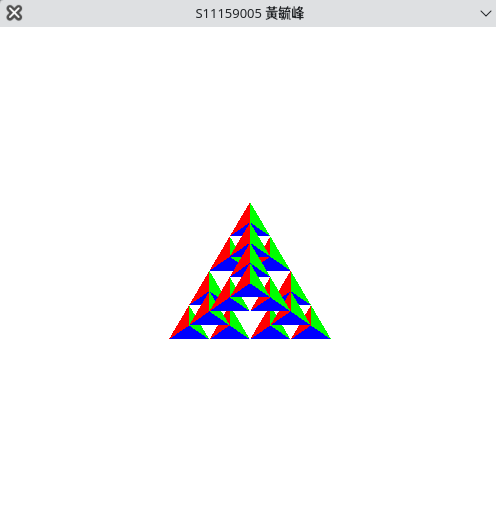
\includegraphics[width=0.8\textwidth]{img/hw2_result.png}
  \caption{執行結果}
\end{figure}

\newpage
\section*{心得}
在這次的作業中,我學習到了許多關於 3D 圖形繪製的重要概念,
不僅提升了我的程式設計能力,也加深了我對電腦圖學的興趣,
此外為了能夠在不依靠其他 libraby 情況下做出選單,
繪製並處理點擊事件花了許多的時間。

\section*{SourceCode}
\sloppy
\noindent \url{https://github.com/IDK-Silver/NUTN-CSIE-Code/tree/main/ComputerGraphics/hw1}





\end{document}
